% ============================================================
% リソグラフィー工程における高次補正の回帰手法（技術レポート）
% Overleaf: メニュー → Compiler を「LuaLaTeX」にしてコンパイルする
% 図は figures/ フォルダに置く（sim/make_figures.m で生成）
% ============================================================
\documentclass[11pt,a4paper]{ltjsarticle}
\usepackage{amsmath,amssymb,bm}
\usepackage{graphicx}
\usepackage{booktabs}
\usepackage[margin=25mm]{geometry}
\usepackage[hidelinks]{hyperref}

\begin{document}

% ------------------------------------------------------------
% 表紙
% ------------------------------------------------------------
\begin{titlepage}
  \centering
  \vspace*{45mm}
  {\LARGE\bfseries リソグラフィー工程における\\[3mm]高次補正の回帰手法に関する検討\par}
  \vspace{8mm}
  {\large ―VIFによる補正項選定・ロバスト回帰・正則化―\par}
  \vspace{45mm}
  {\Large 著者名\par}  % ← 著者名を記入する
  \vspace{8mm}
  {\large \today\par}
  \vfill
\end{titlepage}

% ------------------------------------------------------------
% 目次
% ------------------------------------------------------------
\tableofcontents
\newpage

% ============================================================
\section{序論}
% ============================================================

\subsection{プロセス微細化と重ね合わせにおける動向}

半導体デバイスの微細化に伴い，層間の重ね合わせ誤差（オーバーレイ）は歩留まりを左右する主要因になっている．
ITRS 2006年版のリソグラフィ章では，「マスク描画位置を含む多重露光のオーバーレイ」が最も困難な課題の筆頭に挙げられた\cite{Adel2007}．
この傾向は現在も続いている．IBMのロードマップでは，エッジ配置誤差（EPE）を現状の約3.0\,nmから約1.2\,nmへ縮小する目標が示されている\cite{Gabor2026}．
計測の分野でもサブナノメートルのオーバーレイ時代に入ったとの認識が共有されており\cite{Klein2026}，3D NANDやウェハ接合などの新しいデバイス構造が，計測ターゲットの配置や信号品質に新たな制約を加えている\cite{Katz2026}．

オーバーレイ誤差は古くから，並進・回転・倍率・台形・レンズディストーションといった成分に分解して記述されてきた\cite{MacMillen1982}．
量産の制御では，ウェハ（Shot配列）側4項，Shot内側4項，並進2項からなる10パラメータの線形モデルをRun-to-Run（R2R）で制御する方式が長く標準であった\cite{Duclaux2020}．
しかし，ウェハあたり10〜20 Shot，Shotあたり4〜5点を計測する線形モデルでは，3x/2x\,nm世代の要求を満たせないことが示されている\cite{Huang2012FxFc}．

Shot内の非線形な誤差は，レチクル加熱\cite{Lim2014}，照明条件の違いによるレンズディストーション\cite{Pike2015}，投影レンズの熱収差\cite{Matsuyama2015,Ishiyama2016}，ウェハ内で変化するレンズ・レチクル加熱\cite{Chen2018}など，複数の物理現象から生じる．
これらは線形項だけでは表現できないため，2次以上の多項式項を用いる高次補正が必要になる．

\subsection{近年の高次補正について}

高次補正は，Shot配列（ウェハ格子）に対するHOPC（High Order Process Correction），Shot内に対するiHOPC（intra-field HOPC），Shotごとに補正値を持つCPE（Correction Per Exposure）に大別される．
Huangらは40\,nm世代のDRAMでiHOPCとCPEを評価し，オーバーレイを70\,\%改善して，ウェハ全面計測の平均$+3\sigma$を6〜5\,nm程度に抑えた\cite{Huang2009}．
Chiuらは，iHOPCの3次項の一部とCPEを併用する構成が最良であり，計測サンプリングを最適化すれば計測装置の使用時間を26\,\%削減しても歩留まりを維持できることを示した\cite{Chiu2012}．
補正能力そのものを高める提案もある．Ruiらはレチクル周辺のアクチュエータで5次までの歪みを補償する方式を有限要素シミュレーションで検討し，1・2次でほぼ100\,\%，3・4次で80\,\%超，5次で68.16\,\%の補正率を報告している\cite{Rui2025}．

一方で，補正項の増加はモデルの安定性という新しい問題を生む．
高次の多項式項は互いに強く相関し，測定誤差の影響を増幅するためである\cite{Ullah2013}．
これに対して，直交基底であるZernike多項式への置き換え\cite{Ju2016}，Lasso回帰による補正項の自動選択\cite{Ehrlich2025,Ehrlich2026}，モデルを仮定しない主成分分析\cite{Mohammad2026}などが提案されている．
また，計測誤差への感度が顕著になるのは，サンプリング密度が低く項数の多いモデルに限られることも報告されている\cite{Klein2026}．
つまり高次補正では，計測装置の性能だけでなく，補正式の項の選び方と回帰計算の方法が補正精度を左右する．

本報告では，ASML社およびニコン社のShot高次補正演算式を題材に，回帰計算で生じる課題（異常値，測定誤差，多重共線性，オーバーフィッティング）を整理する．
そのうえで，(1) VIF（分散拡大係数）による補正項（kパラメータ）の事前選定，(2) ロバスト回帰，(3) 正則化の3つを組み合わせた回帰手法を提案し，乱数で生成した1000通りのShotを用いたシミュレーションでその有効性を評価する．

% ============================================================
\section{高次補正}
% ============================================================

\subsection{論文に見る高次補正の事例}

\subsubsection{高次補正の回帰計算}

Shot中心を原点とするマーク座標を$(x,y)$，その点で測定されたオーバーレイを$(d_x,d_y)$とする．
ASML社のiHOPCでは，3次までの多項式で次のように表す\cite{Huang2009,Duclaux2020}．
\begin{align}
  d_x &= k_1 + k_3x + k_5y + k_7x^2 + k_9xy + k_{11}y^2 + k_{13}x^3 + k_{15}x^2y + k_{17}xy^2 + k_{19}y^3, \label{eq:asml_x}\\
  d_y &= k_2 + k_4y + k_6x + k_8y^2 + k_{10}xy + k_{12}x^2 + k_{14}y^3 + k_{16}xy^2 + k_{18}x^2y + k_{20}x^3. \label{eq:asml_y}
\end{align}
係数$k_1$〜$k_{20}$はkパラメータと呼ばれ，多数のマークの測定値から最小二乗法で求める．
Adelらは同じ3次形式をウェハ格子とShot内の両方に適用した例を示し，具体的な項の構成は露光装置によって異なると述べている\cite{Adel2007}．
実運用ではすべての項を使うとは限らない．Duclauxらは線形項に9つの高次項を加えた15項のiHOPCをR2Rで運用し\cite{Duclaux2020}，Chiuらは3次項の一部だけを用いている\cite{Chiu2012}．
ニコン社の露光装置でも，オーバーレイ最適化ソフトウェアによってウェハ格子を5次，Shotを3次までの関数で補正でき，Shotごとの格子はマップで補償することもできる\cite{Matsuyama2015}．

回帰計算は，係数ベクトル$\bm\beta$と設計行列$X$（各行が1つのマーク，各列が1つの項）を用いて
\begin{equation}
  \bm y = X\bm\beta + \bm\varepsilon,\qquad
  \hat{\bm\beta}_{\mathrm{OLS}} = (X^\top X)^{-1}X^\top\bm y
  \label{eq:ols}
\end{equation}
と書ける．ここで$\bm y$は測定値，$\bm\varepsilon$は測定誤差であり，$d_x$と$d_y$は別々の式として回帰する．

\subsubsection{KLAによるZernike多項式の提案}

JuらはSK hynixとKLA-Tencor（現KLA）の共同研究として，ウェハ格子の項をZernike多項式で表し，APCの平滑化計算をZernike基底で行う方式を量産環境で評価した\cite{Ju2016}．
Zernike多項式は単位円上で直交するため，項どうしの共線性が下がり，補正値の変動が抑えられる．
従来のXY多項式と同じ表現力をもつ3次のZernikeモデルを用いた結果，オーバーレイ変動が7\,\%，線形モデル項の変動が22\,\%減少し，$|\text{平均}|+3\sigma$がX方向で5\,\%，Y方向で7\,\%改善して，歩留まりが約0.1\,\%向上した．
ただし，Shot内の項は従来のXY多項式のまま扱っており，APCで計算した係数は最終的にXY多項式へ変換して露光装置へ送られる．
なお松山も，投影レンズの制御の文脈で，Fringe Zernike関数を組み合わせた直交なディストーション関数を提案している\cite{Matsuyama2015}．

\subsubsection{正則化の事例}

Ehrlichら（KLA）は，Lasso回帰（L1正則化）\cite{Tibshirani1996}と計測データ向けの交差検証を組み合わせ，多項式モデルから有意な項を自動選択する手法を提案した\cite{Ehrlich2025}．
目的関数は
\begin{equation}
  \min_{\beta_0,\bm\beta}\ \frac{1}{N}\sum_{i=1}^{N}\left(y_i-\beta_0-\bm x_i^\top\bm\beta\right)^2+\lambda\sum_{j=1}^{p}|\beta_j|
  \label{eq:lasso_ehrlich}
\end{equation}
であり，正則化パラメータ$\lambda$は，外側がウェハ単位のleave-one-out，内側がマーク単位の$k$分割という入れ子の交差検証で決める．
選ばれた項は，最後に正則化なしの最小二乗法で当てはめ直す．
R2R制御のシミュレーションでは，13次Zernikeモデル（105項）や固定の2次モデルより低いCD均一性が得られた．
続報では同じ手法をトラックモジュールの文脈ごとに適用し，105項の候補を文脈グループあたり最大22項まで絞り込んでいる\cite{Ehrlich2026}．

\subsection{高次補正における回帰の課題}

\subsubsection{異常値}

重ね合わせ計測では，ターゲットの欠陥や異物，信号不良により，他の点から大きく外れた測定値（フライヤー）が混入する．
量産の制御でも，モデル計算の前にフライヤーを除去する処理が組み込まれている\cite{Lee2017}．
最小二乗法は残差の二乗和を最小にするため，1点の異常値でも推定値を大きく動かす．
高次項を含むモデルは局所的な変形を表す自由度が高いため，異常値に引きずられて，本来存在しない高次の歪みを推定しやすい．

\subsubsection{測定誤差}

測定値に独立な誤差$\varepsilon_i\sim N(0,\sigma^2)$が含まれるとき，最小二乗推定量の分散は
\begin{equation}
  \mathrm{Var}(\hat{\bm\beta}_{\mathrm{OLS}})=\sigma^2(X^\top X)^{-1}
  \label{eq:var}
\end{equation}
となる．
近年の計測装置の総合計測不確かさ（TMU）は0.3\,nmを下回る水準にあるが\cite{Klein2026}，マーク数に対して項数が多く$(X^\top X)^{-1}$が大きい場合には，小さな測定誤差でも補正係数へ大きく伝わる．

\subsubsection{多重共線性}

高次の多項式項は同じ座標のべき乗であるため，互いに相関しやすい．
Ullahらのシミュレーションでは，線形モデルの項間相関はすべて0.25未満であったのに対し，3次多項式モデルでは49\,\%の組み合わせが0.25を，22\,\%が0.5を超え，線形の倍率と3次の倍率の間には$-0.9$より強い負の相関があった\cite{Ullah2013}．
共線性が強いと$X^\top X$が特異に近づき，式\eqref{eq:var}の分散が大きくなる．
その結果，高次項だけでなく線形項まで不安定になり，R2R制御の予測精度が低下する\cite{Ullah2013,Ju2016}．

\subsubsection{オーバーフィッティング}

項数がマーク数に近づくと，モデルは測定誤差まで表現してしまう．
このとき測定点での残差は小さく見えるが，測定していない位置での補正誤差はかえって大きくなる．
Shotごとに19項を当てはめるCPEモデルは，ウェハ端の変形をよく捉える一方で広いサンプリングを必要とし，雑音とオーバーフィッティングの影響を受けやすい\cite{Lee2017}．
Ehrlichらも，不要な項を含むモデルは過学習を起こし，制御ループの安定性を下げると指摘している\cite{Ehrlich2025}．

% ============================================================
\section{提案手法}
% ============================================================

本報告では，次の3つを組み合わせた回帰手法を提案する．
\begin{enumerate}
  \item VIFにより，強い共線性をもつ補正項を回帰の前に削除する（\ref{sec:vif}節）．
  \item Huber損失によるロバスト回帰で，異常値の影響を抑える（\ref{sec:robust}節）．
  \item L1またはL2正則化で，補正係数の分散を抑える（\ref{sec:reg}節）．
\end{enumerate}

\subsection{VIFによるkパラメータ選定}\label{sec:vif}

項$j$の分散拡大係数（VIF）は，項$j$の列を他の項（切片を含む）で回帰したときの決定係数$R_j^2$を用いて
\begin{equation}
  \mathrm{VIF}_j=\frac{1}{1-R_j^2}
  \label{eq:vif}
\end{equation}
で定義される\cite{Marquardt1970}．
係数$\hat\beta_j$の分散は，その項が他の項と無相関な場合の$\mathrm{VIF}_j$倍になる．
VIFはマーク配置と項の組み合わせだけで決まり，測定値には依存しないため，補正式の設計段階で評価できる．

削除の手順を次に示す．しきい値には一般的な目安である$\mathrm{VIF}=10$を用いる．
\begin{enumerate}
  \item 切片と1次項（並進・倍率・回転）は物理的に必須なので，削除の対象から除く．
  \item すべての項のVIFがしきい値未満なら終了する．
  \item VIFがしきい値以上の高次項があれば，その中で次数が最も高い項（同じ次数ならVIFが最大の項）を削除する．
        しきい値以上の項が1次項だけの場合は，高次項の中でVIFが最大の項を削除する．
  \item 残った項でVIFを計算し直し，2.に戻る．
\end{enumerate}
手順3で次数を優先するのは，VIFが最大の項を単純に削除すると，$y^3$を削除して$y^6$を残すような，多項式の階層性に反する選択が起こるためである．

\subsection{ロバスト回帰}\label{sec:robust}

Huberは，残差が小さい範囲では二乗で，大きい範囲では絶対値で増える損失関数
\begin{equation}
  \rho_c(u)=
  \begin{cases}
    u^2/2 & (|u|\le c)\\
    c|u|-c^2/2 & (|u|>c)
  \end{cases}
  \label{eq:huber}
\end{equation}
を提案した\cite{Huber1964}．
残差$r_i=y_i-\bm x_i^\top\bm\beta$を尺度$s$で割った$u_i=r_i/s$について$\sum_i\rho_c(u_i)$を最小化すると，外れた点の影響は残差に比例してしか増えないため，異常値に強い推定が得られる．
$c=1.345$は，誤差が正規分布に従うときに最小二乗法の95\,\%の効率を保つ値である．
尺度には残差の中央値絶対偏差（MAD）から求めた$s=1.4826\,\mathrm{median}_i\left|r_i-\mathrm{median}(\bm r)\right|$を用いる．

最小化には反復再重み付け最小二乗法（IRLS）\cite{Holland1977}を用いる．
各マークの重み
\begin{equation}
  w_i=\min\left(1,\ \frac{c\,s}{|r_i|}\right)
  \label{eq:weight}
\end{equation}
を計算し，重み付き最小二乗問題を解き直す操作を，係数が収束するまで繰り返す．初期値には最小二乗解を用いる．

\subsection{正則化}\label{sec:reg}

係数の大きさに罰則を加えると，推定値にわずかな偏りを許す代わりに分散を減らせる．
L2正則化（リッジ回帰）\cite{Hoerl1970}とL1正則化（Lasso）\cite{Tibshirani1996}を，ロバスト回帰の重み$w_i$と組み合わせた目的関数を次のように定める．
\begin{align}
  \text{L2：}\quad &\min_{\bm\beta}\ \frac{1}{2n}\sum_{i=1}^{n}w_i\left(y_i-\bm x_i^\top\bm\beta\right)^2+\frac{\lambda_2}{2}\sum_{j\in\mathcal H}\beta_j^2, \label{eq:ridge}\\
  \text{L1：}\quad &\min_{\bm\beta}\ \frac{1}{2n}\sum_{i=1}^{n}w_i\left(y_i-\bm x_i^\top\bm\beta\right)^2+\lambda_1\sum_{j\in\mathcal H}|\beta_j|. \label{eq:l1}
\end{align}
ここで$n$はマーク数，$\mathcal H$は2次以上の項の集合である．
並進・倍率・回転は常に存在する大きな成分なので罰則をかけない．
罰則の効き方を項の間でそろえるため，切片以外の列はマーク位置で平均0，標準偏差1に標準化してから回帰する．
ロバスト回帰を組み合わせない場合は$w_i=1$とする．
L2は線形方程式として直接解け，L1は座標降下法\cite{Friedman2010}で解く．
L2は相関した項の係数をそろって縮小するのに対し，L1は係数を厳密に0にして項を選択する．
ただしL1には，強く相関した項の中から1つをほぼ任意に選ぶ傾向がある\cite{Zou2005}．

% ============================================================
\section{実験}
% ============================================================

\subsection{Shotと計測マークの設定}

Shotの大きさを$26\times33$\,mm（$x$：スリット方向，$y$：スキャン方向）とし，Shot中心を原点とした．
計測マークは$x=-12,-6,0,6,12$\,mm，$y$は$-15.5$\,mmから$15.5$\,mmまでの等間隔7行とし，計$5\times7=35$点に配置した．
回帰では，座標をShotの半幅13\,mmと半高さ16.5\,mmで割り，Shot端で$\pm1$となる正規化座標を用いた．
補正の良さは，Shot全面を覆う$21\times21$点の評価グリッドで判定した．
生成したShotとマーク配置の例を図\ref{fig:example}に示す．

\begin{figure}[tb]
  \centering
  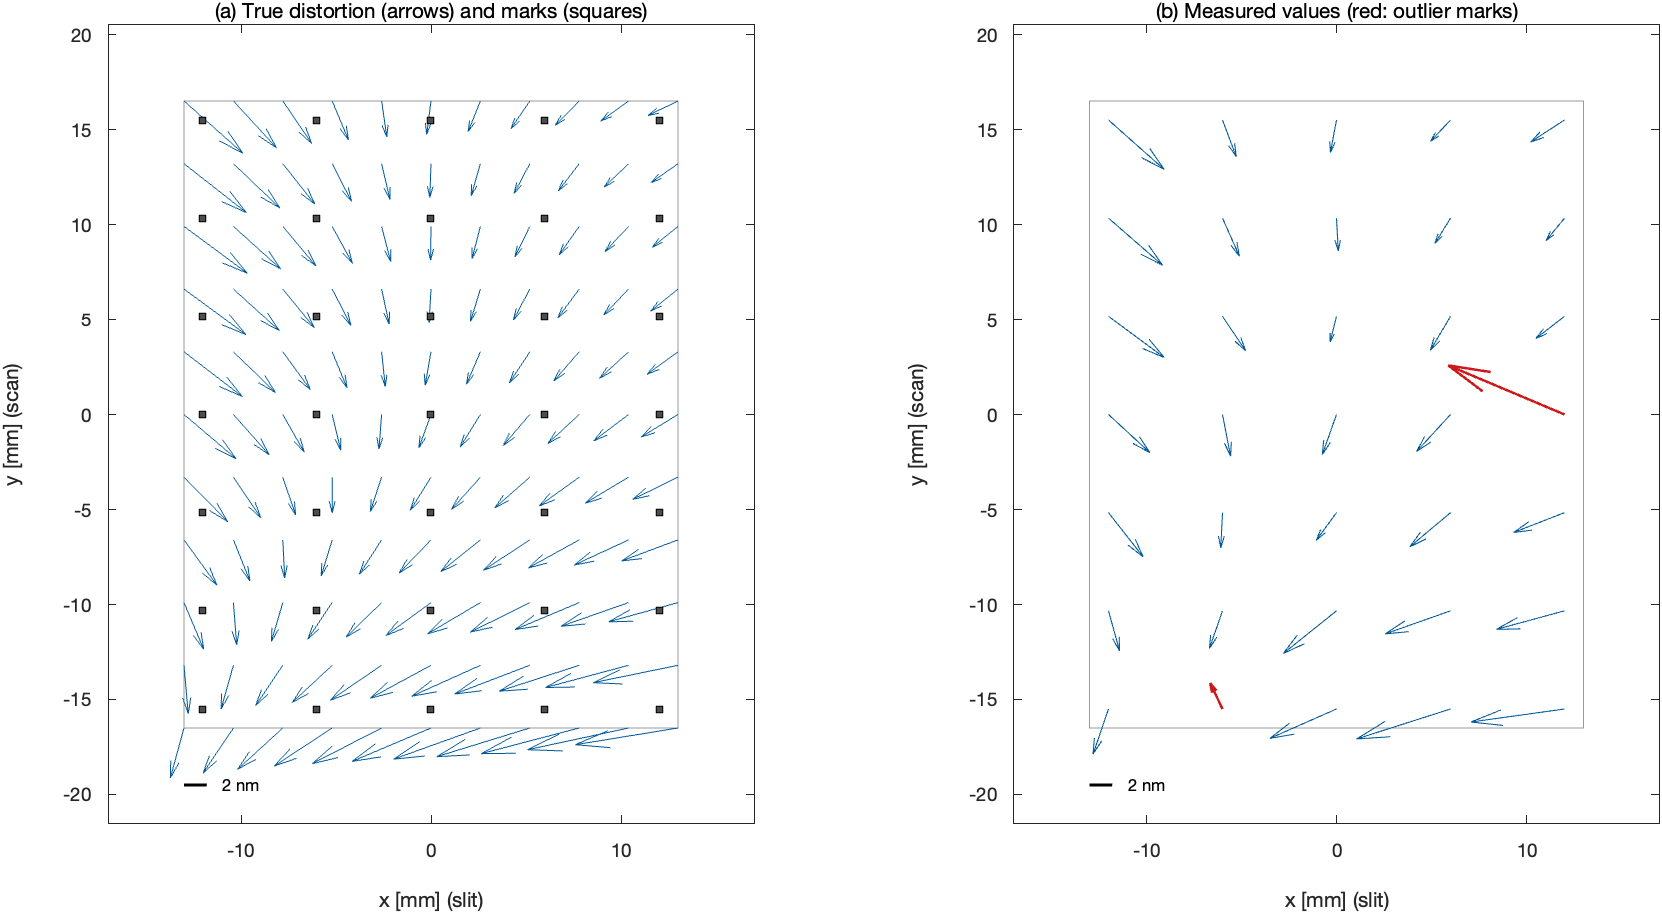
\includegraphics[width=\linewidth]{figures/fig_shot_example}
  \caption{生成したShotの例．(a) 真の歪み（矢印，評価グリッドを1点おきに表示）とマーク配置（四角）．(b) マーク位置での測定値（赤は異常値を含むマーク）．}
  \label{fig:example}
\end{figure}

\subsection{乱数による高次歪みをもったShotの生成}

真の歪みは，後述するASML式とニコン式の項をすべて含む多項式（$d_x$は13項，$d_y$は16項）とし，各係数を次数ごとに表\ref{tab:truth}の条件で乱数生成した．
係数は正規化座標での値なので，Shot端での変位量の目安になる．
実際のShotでは高次成分がすべて同時に現れるとは限らないため，2次以上の項には出現確率を設けた．
これを1000回繰り返し，互いに独立な1000通りのShotを作成した．乱数のシードは固定しており，結果は再現できる．

\begin{table}[tb]
  \centering
  \caption{真の歪み係数の生成条件（係数は平均0の正規乱数）}
  \label{tab:truth}
  \begin{tabular}{lccccc}
    \toprule
    次数 & 0（並進） & 1（倍率・回転） & 2 & 3 & 4〜6 \\
    \midrule
    標準偏差 [nm] & 2.0 & 2.0 & 0.8 & 0.6 & 0.4 \\
    出現確率      & 1.0 & 1.0 & 0.5 & 0.5 & 0.3 \\
    \bottomrule
  \end{tabular}
\end{table}

\subsection{測定誤差の付与}

マーク位置の真値に，標準偏差0.3\,nmの正規乱数を$d_x$，$d_y$それぞれ独立に加えた．
この値は近年の計測装置のTMUの水準\cite{Klein2026}を想定したものである．
さらに各マークを確率5\,\%で異常マークとし，そのマークの$d_x$と$d_y$に大きさ3〜8\,nm（符号はランダム）の誤差を加えた．
1 Shotあたりの異常マークは平均1.75点である．
比較のため，異常値を加えない条件も同じ乱数で作成した．以下，前者を「異常値あり」，後者を「異常値なし」と呼ぶ．

\subsection{ASML・ニコン社のShot高次補正演算式でのVIF算出}

ASML式は式\eqref{eq:asml_x}，\eqref{eq:asml_y}の各10項である．
ニコン式は，Shot線形成分（並進・倍率・回転）に高次の係数を加えた次の形とした．
\begin{align}
  d_x &= c_{00}+c_{10}x+c_{01}y+\sum_{(m,n)\in\mathcal S_x}c_{mn}\,x^my^n, \label{eq:nikon_x}\\
  d_y &= e_{00}+e_{01}y+e_{10}x+\sum_{(m,n)\in\mathcal S_y}e_{mn}\,x^my^n, \label{eq:nikon_y}
\end{align}
\begin{align*}
  \mathcal S_x&=\{(0,2),(0,3),(0,4),(0,5),(0,6),(2,0),(3,0),(1,1),(1,2)\},\\
  \mathcal S_y&=\{(1,1),(0,2),(1,2),(0,3),(1,3),(0,4),(1,4),(0,5),(1,5),(0,6),(2,0),(2,1)\}.
\end{align*}
$d_x$は12項，$d_y$は15項であり，スキャン方向$y$について6次までの項をもつ点がASML式と大きく異なる．
この項構成は，ニコン社の露光装置が出力するShot高次補正係数の組に基づき，係数名の添字$mn$を$x^my^n$の次数と解釈して作成した．
この対応は装置仕様での確認を要する．
また，$y$について6次の項を解くにはスキャン方向に7行以上のマークが必要であり，本実験のマーク配置（7行）はこの条件を満たす最小の構成である．

各式について，35点のマーク配置で式\eqref{eq:vif}のVIFを計算し，\ref{sec:vif}節の手順で項を削除した．
削除後の式を，それぞれ「ASML-VIF」「Nikon-VIF」と呼ぶ．

\subsection{ロバスト回帰と正則化の演算条件}

回帰手法は，最小二乗法（OLS），Huber回帰（Huber），L2正則化（L2），L1正則化（L1），ロバスト回帰と正則化の組み合わせ（Huber+L2，Huber+L1）の6種類とした．
ハイパーパラメータは全Shotで固定し，交差検証などによる調整は行っていない．
\begin{itemize}
  \item L1：$\lambda_1=\sigma/\sqrt{n}=0.3/\sqrt{35}\approx0.051$\,nm．標準化した直交な項であれば，係数の標準誤差1個分を打ち切る強さである．
  \item L2：$\lambda_2=0.1$．標準化した直交な項であれば，係数を$1/(1+\lambda_2)\approx0.91$倍に縮小する強さである．
  \item Huber：$c=1.345$．IRLSは最大50回とし，係数の変化が$10^{-5}$\,nm未満になった時点で収束とした．
\end{itemize}
4種類の補正式（ASML，ASML-VIF，Nikon，Nikon-VIF）と6種類の回帰手法を組み合わせた24条件を，異常値あり・なしの両方で評価した．
計算にはMATLAB R2022bを用いた．

\subsection{評価方法}

各条件で推定した係数から評価グリッド上の補正値を計算し，真の歪みとの差（補正残差）のRMSをShotごとに求めた．
この値は，測定点での当てはまりではなく，Shot全面で補正後に残る誤差を表す．
1000 Shotの分布は，中央値，95パーセンタイル，全Shot・全評価点をまとめた$|\text{平均}|+3\sigma$で要約した．
$d_x$と$d_y$は別々に評価した．
2つの条件を比べる場合は，Shotごとに$d_x$と$d_y$の残差RMSを二乗平均して1つの値にまとめ，同じShotどうしで比較した．
条件Aの残差が条件Bより小さいShotの割合を「勝率」と呼ぶ．
参考として，雑音のない真値を評価グリッドの全点で当てはめたときの残差（その補正式で表現できる限界．以下「表現限界」）も計算した．

% ============================================================
\section{結果}
% ============================================================
% 表の数値は sim/write_tex_tables.m が results/tex/ に出力した行をそのまま使っている

\subsection{VIFによるkパラメータ選定の結果}

各補正式の項のVIFを図\ref{fig:vif}に，削除の結果を表\ref{tab:vif}に示す．

ASML式では，$d_x$，$d_y$ともに1次項$x$のVIFが10.4とわずかにしきい値を超えた．
これは$x$が$x^3$（VIF 9.0）や$xy^2$と相関するためであり，手順に従って$x^3$（$d_x$では$k_{13}$，$d_y$では$k_{20}$）を削除すると，最大VIFは8.8に下がった．

ニコン式では，スキャン方向$y$のべき乗項どうしの共線性がきわめて強く，VIFは$y^4$で2541.5，$y^6$で1267.0，$y^3$で322.6に達した．
7行しかないマークの$y$座標に対して，$y^2$から$y^6$までのべき乗を同時に当てはめるためである．
次数の高い項から削除した結果，$d_x$は12項から8項（$y^6$，$y^5$，$y^4$，$x^3$を削除），$d_y$は15項から10項（$y^6$，$xy^5$，$y^5$，$xy^4$，$y^4$を削除）となり，最大VIFはそれぞれ7.4と8.8に下がった．

\begin{figure}[tb]
  \centering
  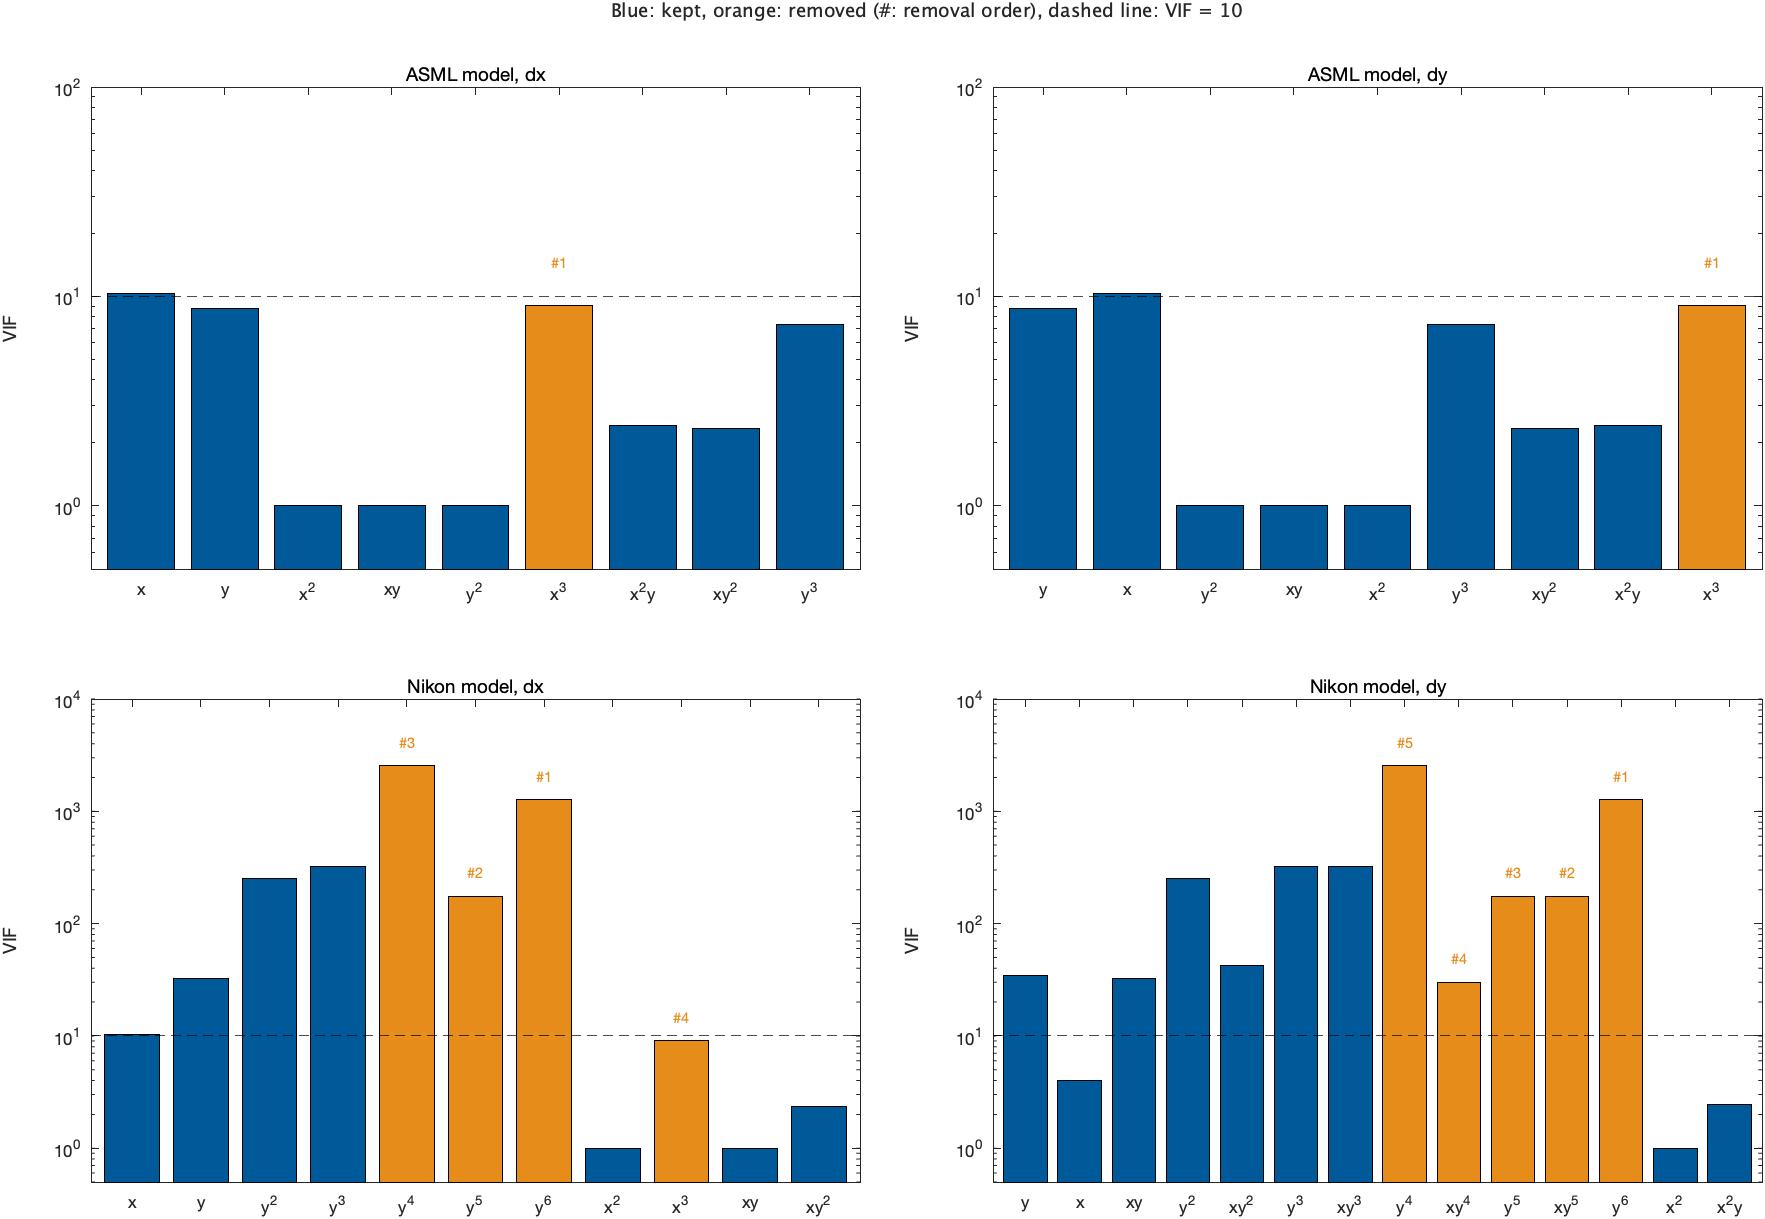
\includegraphics[width=\linewidth]{figures/fig_vif}
  \caption{35点のマーク配置で計算した各項のVIF（縦軸は対数）．上段がASML式，下段がニコン式．橙は\ref{sec:vif}節の手順で削除した項，\#は削除した順番，破線はしきい値（VIF $=10$）を表す．}
  \label{fig:vif}
\end{figure}

\begin{table}[tb]
  \centering
  \caption{VIFによるkパラメータ削除の結果}
  \label{tab:vif}
  \begin{tabular}{llclcc}
    \toprule
    補正式 & 軸 & 項数 & 削除した項（削除した順） & 最大VIF（削除前） & 最大VIF（削除後） \\
    \midrule
    ASML & $d_x$ & 10 $\to$ 9 & $x^{3}$ & 10.4 & 8.8 \\
    ASML & $d_y$ & 10 $\to$ 9 & $x^{3}$ & 10.4 & 8.8 \\
    Nikon & $d_x$ & 12 $\to$ 8 & $y^{6}$, $y^{5}$, $y^{4}$, $x^{3}$ & 2541.5 & 7.4 \\
    Nikon & $d_y$ & 15 $\to$ 10 & $y^{6}$, $xy^{5}$, $y^{5}$, $xy^{4}$, $y^{4}$ & 2541.5 & 8.8 \\
    \bottomrule
  \end{tabular}
\end{table}

\subsection{補正残差の比較}

異常値ありの条件におけるShot全面の補正残差RMSを表\ref{tab:summary}と図\ref{fig:box}に，参考値を表\ref{tab:reference}に示す．
補正前の歪みは，RMSの中央値で約2.3\,nmである．

最小二乗法（OLS）では，残差の中央値がASML式で0.59〜0.60\,nm，ニコン式で0.91〜1.02\,nmとなり，項数の多いニコン式ほど悪化した．
正則化だけを加えても（L2，L1），残差の中央値は0.46〜0.54\,nmにとどまった．
一方，Huber回帰を用いると，ASML式，ASML-VIF式，Nikon-VIF式の残差の中央値は0.18〜0.20\,nmまで下がった．
削除前のニコン式では，Huber回帰でも中央値が0.28〜0.34\,nmであり，特に$d_y$の95パーセンタイルが1.07\,nmと大きかった．

すべての補正式で残差の中央値が最小になった手法はHuber+L2であり，中央値は0.16〜0.18\,nm，$|\text{平均}|+3\sigma$は0.55〜0.65\,nmであった．
これはOLSの$|\text{平均}|+3\sigma$（ASML式で2.00〜2.03\,nm，ニコン式で3.30〜3.60\,nm）の約1/4〜1/6である．
なお，雑音のない真値に対する表現限界（表\ref{tab:reference}）は，中央値で削除前の補正式が0.04\,nm以下，VIFで削除した補正式でも0.08\,nm以下であった．
したがって，いずれの条件でも残差の大部分は，測定誤差と異常値に起因する推定誤差である．

\begin{table}[tb]
  \centering
  \caption{異常値ありの条件における補正残差RMS [nm]（1000 Shot）．補正式の下の括弧は$d_x$/$d_y$の項数，太字は各補正式の中で中央値が最小の手法を表す．}
  \label{tab:summary}
  \small
  \begin{tabular}{llcccccc}
    \toprule
     & & \multicolumn{3}{c}{$d_x$} & \multicolumn{3}{c}{$d_y$} \\
    \cmidrule(lr){3-5}\cmidrule(lr){6-8}
    補正式 & 手法 & 中央値 & 95\,\% & $|\text{平均}|+3\sigma$ & 中央値 & 95\,\% & $|\text{平均}|+3\sigma$ \\
    \midrule
    ASML & OLS & 0.591 & 1.091 & 1.998 & 0.596 & 1.131 & 2.026 \\
    (10/10) & Huber & 0.183 & 0.335 & 0.677 & 0.185 & 0.363 & 0.717 \\
     & L2 & 0.501 & 0.919 & 1.713 & 0.505 & 0.957 & 1.742 \\
     & L1 & 0.481 & 0.957 & 1.703 & 0.488 & 0.992 & 1.739 \\
     & Huber+L2 & \textbf{0.164} & 0.268 & 0.545 & \textbf{0.169} & 0.277 & 0.560 \\
     & Huber+L1 & 0.180 & 0.294 & 0.595 & 0.188 & 0.301 & 0.614 \\
    \midrule
    ASML-VIF & OLS & 0.549 & 1.029 & 1.888 & 0.557 & 1.073 & 1.911 \\
    (9/9) & Huber & 0.182 & 0.346 & 0.675 & 0.188 & 0.370 & 0.713 \\
     & L2 & 0.490 & 0.908 & 1.685 & 0.498 & 0.940 & 1.713 \\
     & L1 & 0.467 & 0.920 & 1.665 & 0.479 & 0.966 & 1.696 \\
     & Huber+L2 & \textbf{0.168} & 0.289 & 0.572 & \textbf{0.176} & 0.298 & 0.586 \\
     & Huber+L1 & 0.181 & 0.302 & 0.603 & 0.191 & 0.305 & 0.620 \\
    \midrule
    Nikon & OLS & 0.912 & 1.961 & 3.304 & 1.016 & 2.078 & 3.597 \\
    (12/15) & Huber & 0.279 & 0.547 & 1.149 & 0.343 & 1.069 & 1.644 \\
     & L2 & 0.515 & 0.943 & 1.747 & 0.535 & 1.032 & 1.860 \\
     & L1 & 0.483 & 0.952 & 1.719 & 0.504 & 1.056 & 1.816 \\
     & Huber+L2 & \textbf{0.173} & 0.292 & 0.581 & \textbf{0.181} & 0.342 & 0.645 \\
     & Huber+L1 & 0.182 & 0.320 & 0.611 & 0.184 & 0.304 & 0.607 \\
    \midrule
    Nikon-VIF & OLS & 0.531 & 0.971 & 1.805 & 0.587 & 1.133 & 2.011 \\
    (8/10) & Huber & 0.188 & 0.340 & 0.654 & 0.195 & 0.460 & 0.787 \\
     & L2 & 0.478 & 0.872 & 1.632 & 0.504 & 0.961 & 1.737 \\
     & L1 & 0.460 & 0.876 & 1.614 & 0.483 & 0.997 & 1.725 \\
     & Huber+L2 & \textbf{0.178} & 0.318 & 0.602 & \textbf{0.176} & 0.303 & 0.595 \\
     & Huber+L1 & 0.188 & 0.331 & 0.630 & 0.188 & 0.305 & 0.618 \\
    \bottomrule
  \end{tabular}
\end{table}

\begin{table}[tb]
  \centering
  \caption{参考値：補正なしの歪みと，各補正式の表現限界（雑音のない真値を全面で当てはめた残差）のRMS [nm]}
  \label{tab:reference}
  \begin{tabular}{lcccc}
    \toprule
     & \multicolumn{2}{c}{$d_x$} & \multicolumn{2}{c}{$d_y$} \\
    \cmidrule(lr){2-3}\cmidrule(lr){4-5}
    条件 & 中央値 & 95\,\% & 中央値 & 95\,\% \\
    \midrule
    補正なし & 2.330 & 4.481 & 2.336 & 4.664 \\
    表現限界 ASML & 0.012 & 0.086 & 0.035 & 0.104 \\
    表現限界 ASML-VIF & 0.039 & 0.178 & 0.057 & 0.178 \\
    表現限界 Nikon & 0.004 & 0.188 & 0.001 & 0.169 \\
    表現限界 Nikon-VIF & 0.076 & 0.232 & 0.042 & 0.176 \\
    \bottomrule
  \end{tabular}
\end{table}

\begin{figure}[tb]
  \centering
  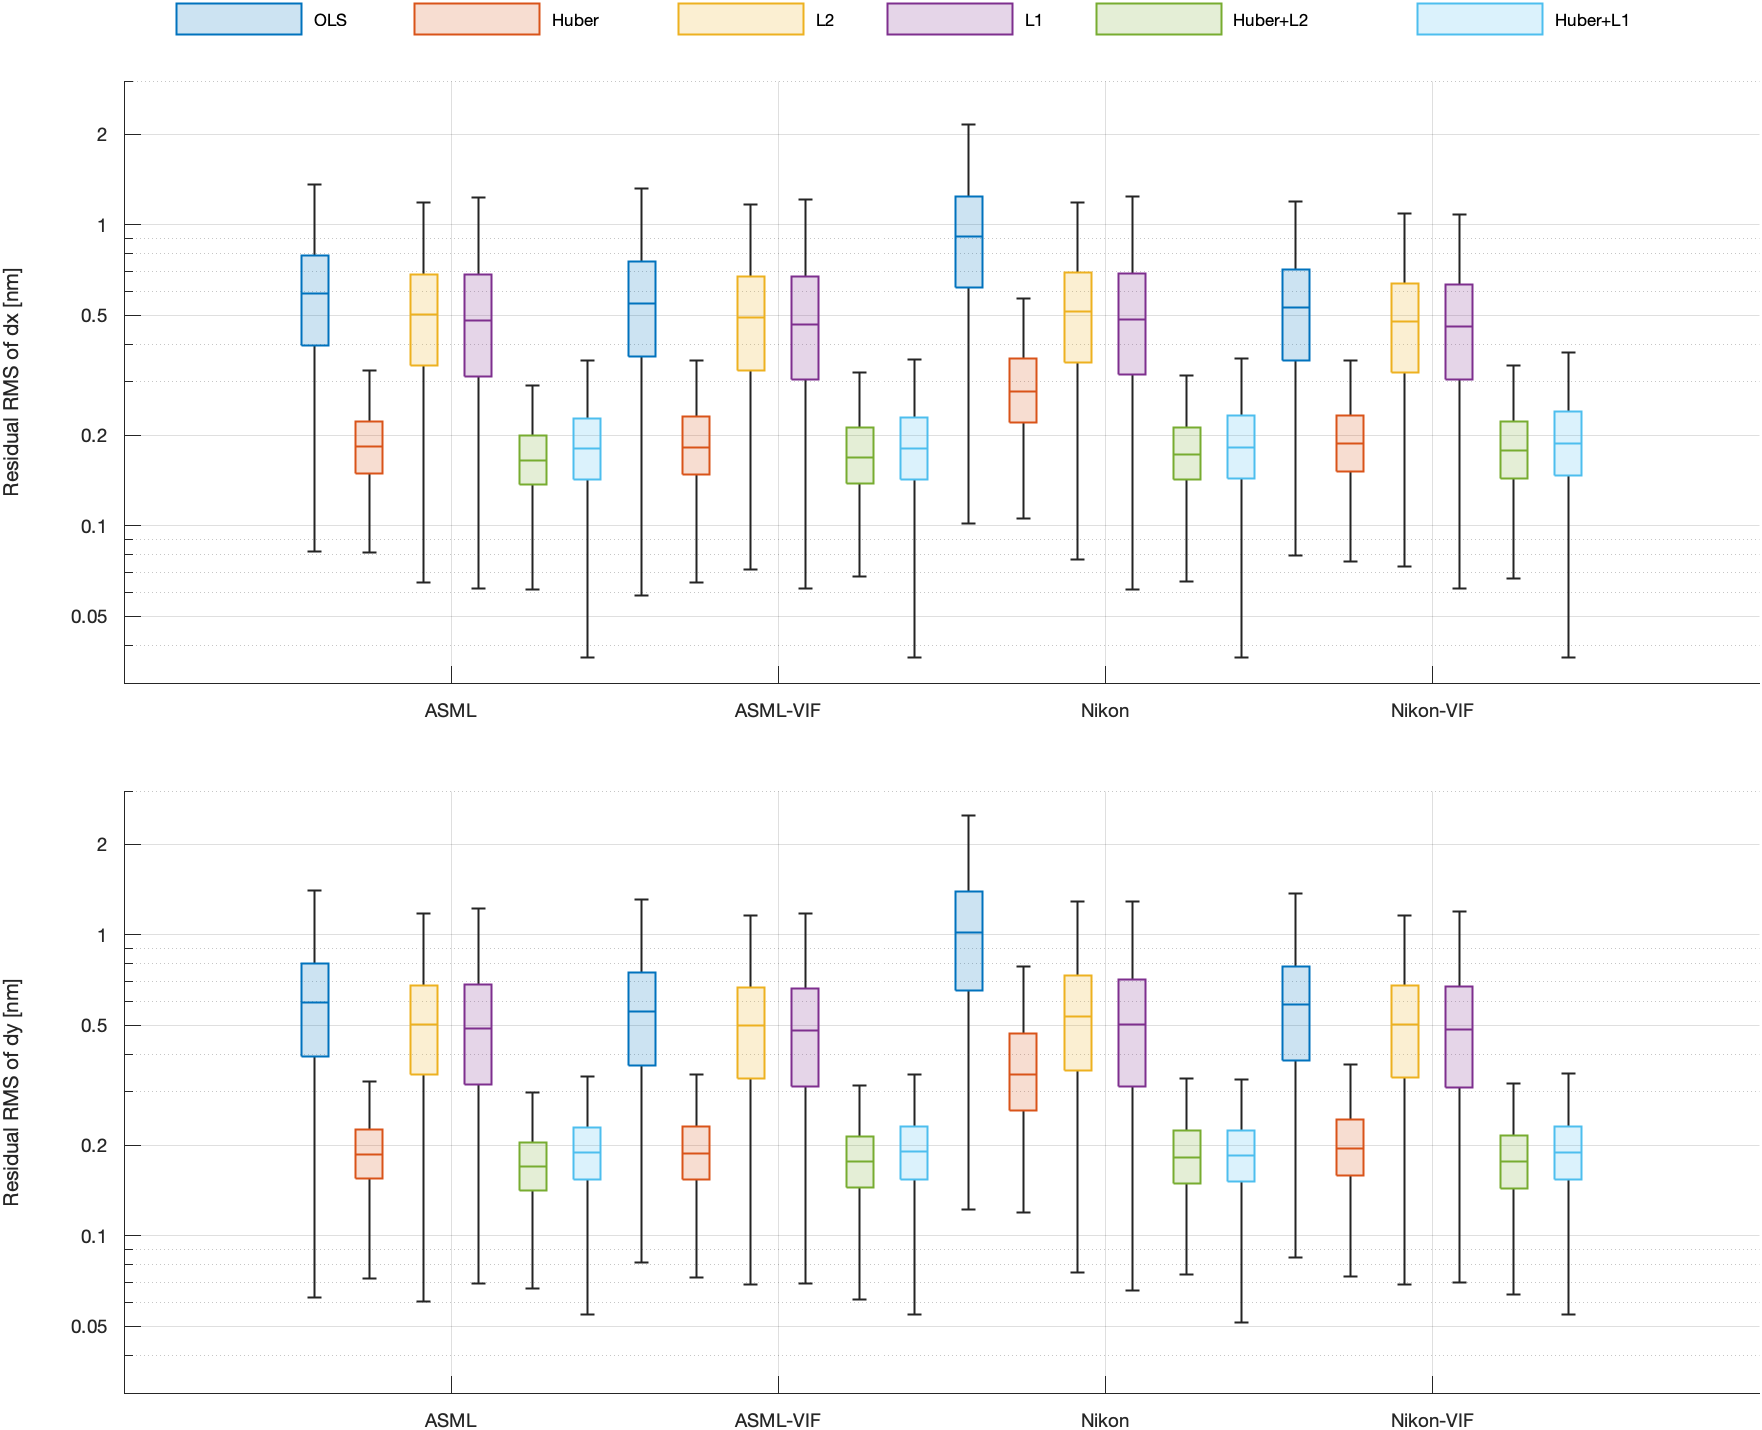
\includegraphics[width=\linewidth]{figures/fig_residual_box}
  \caption{異常値ありの条件における補正残差RMSの分布（1000 Shot，縦軸は対数）．上段が$d_x$，下段が$d_y$．箱は四分位範囲，箱の中の線は中央値，ひげは四分位範囲の1.5倍までの範囲を表す．}
  \label{fig:box}
\end{figure}

\subsection{提案手法の有効性}

提案手法を構成する3つの要素の効果を，同じShotどうしの比較で表\ref{tab:comparison}にまとめる．
低減率は条件Bに対する条件Aの残差中央値の低減割合，勝率は条件Aの残差が条件Bより小さかったShotの割合である．

\paragraph{ロバスト回帰}
Huber回帰は，すべての補正式でOLSに対して残差の中央値を65.8〜69.2\,\%低減し，勝率は89.3〜90.3\,\%であった．
正則化と組み合わせた場合も，L2単独に対して63.2〜65.0\,\%低減した．

\paragraph{VIFによる事前削除}
正則化を用いない場合，ニコン式では事前削除の効果が大きく，残差の中央値がOLSで43.6\,\%，Huber回帰で39.2\,\%低減し，勝率は98\,\%以上であった．
ASML式ではOLSで5.6\,\%低減したが，Huber回帰では差がなかった（$-1.1$\,\%）．
L1正則化と組み合わせた場合，ロバスト回帰を併用しないL1では，事前削除によりASML式で2.4\,\%，ニコン式で4.5\,\%低減した（勝率57.8\,\%，76.6\,\%）．
一方，Huber+L1では事前削除による改善は見られず，ASML式で$-0.9$\,\%（勝率52.0\,\%），ニコン式で$-3.7$\,\%（勝率33.3\,\%）であった．

\paragraph{L2正則化とL1正則化}
事前削除した補正式でHuber回帰と組み合わせた場合，L2はL1より残差の中央値がASML-VIF式で7.9\,\%，Nikon-VIF式で6.1\,\%小さく，勝率は68.8〜70.1\,\%であった．
異常値なしの条件でも，事前削除した補正式ではL2がL1より5.8〜11.3\,\%小さかった．
ただし，ロバスト回帰を併用せずに異常値を含むデータを回帰した場合は，L2のほうが4.1〜4.4\,\%大きかった．
削除前の補正式でも，Huber回帰と組み合わせるとL2がL1より有利であった（ASML式で10.8\,\%，ニコン式で3.3\,\%）．

以上の要素を組み合わせた構成（VIF削除＋Huber回帰＋L2正則化）は，現行の最小二乗法（削除なし）に比べて，残差の中央値をASML式で70\,\%（0.603\,nmから0.178\,nm），ニコン式で82\,\%（1.024\,nmから0.185\,nm）低減した．

\begin{table}[tb]
  \centering
  \caption{同じShotどうしで比べた条件間の差（異常値あり）．A，Bは各条件の残差中央値（$d_x$と$d_y$のRMSを二乗平均した値）[nm]．低減率が正の場合は条件Aが優れる．}
  \label{tab:comparison}
  \footnotesize
  \setlength{\tabcolsep}{3pt}
  \begin{tabular}{lllcccc}
    \toprule
    観点 & 条件A & 条件B & A & B & 低減率[\%] & 勝率[\%] \\
    \midrule
    事前削除（L1併用） & ASML-VIF L1 & ASML L1 & 0.488 & 0.501 & +2.4 & 57.8 \\
     & ASML-VIF Huber+L1 & ASML Huber+L1 & 0.194 & 0.192 & -0.9 & 52.0 \\
     & Nikon-VIF L1 & Nikon L1 & 0.483 & 0.505 & +4.5 & 76.6 \\
     & Nikon-VIF Huber+L1 & Nikon Huber+L1 & 0.197 & 0.191 & -3.7 & 33.3 \\
    \midrule
    L2とL1（削除後） & ASML-VIF L2 & ASML-VIF L1 & 0.509 & 0.488 & -4.1 & 29.5 \\
     & ASML-VIF Huber+L2 & ASML-VIF Huber+L1 & 0.178 & 0.194 & +7.9 & 70.1 \\
     & Nikon-VIF L2 & Nikon-VIF L1 & 0.504 & 0.483 & -4.4 & 31.1 \\
     & Nikon-VIF Huber+L2 & Nikon-VIF Huber+L1 & 0.185 & 0.197 & +6.1 & 68.8 \\
    \midrule
    L2とL1（削除前） & ASML Huber+L2 & ASML Huber+L1 & 0.171 & 0.192 & +10.8 & 75.6 \\
     & Nikon Huber+L2 & Nikon Huber+L1 & 0.184 & 0.191 & +3.3 & 57.8 \\
    \midrule
    ロバスト回帰 & ASML Huber & ASML OLS & 0.186 & 0.603 & +69.2 & 89.3 \\
     & ASML-VIF Huber & ASML-VIF OLS & 0.188 & 0.569 & +67.0 & 89.7 \\
     & Nikon Huber & Nikon OLS & 0.324 & 1.024 & +68.3 & 90.2 \\
     & Nikon-VIF Huber & Nikon-VIF OLS & 0.197 & 0.577 & +65.8 & 90.3 \\
     & ASML-VIF Huber+L2 & ASML-VIF L2 & 0.178 & 0.509 & +65.0 & 89.6 \\
     & Nikon-VIF Huber+L2 & Nikon-VIF L2 & 0.185 & 0.504 & +63.2 & 89.5 \\
    \midrule
    事前削除（正則化なし） & ASML-VIF OLS & ASML OLS & 0.569 & 0.603 & +5.6 & 76.2 \\
     & Nikon-VIF OLS & Nikon OLS & 0.577 & 1.024 & +43.6 & 99.6 \\
     & ASML-VIF Huber & ASML Huber & 0.188 & 0.186 & -1.1 & 56.8 \\
     & Nikon-VIF Huber & Nikon Huber & 0.197 & 0.324 & +39.2 & 98.4 \\
    \bottomrule
  \end{tabular}
\end{table}

% ============================================================
\section{考察}
% ============================================================

\subsection{ロバスト回帰の効果が大きい理由}

本実験の異常値は3〜8\,nmであり，偶然誤差（0.3\,nm）の10倍以上の大きさをもつ．
1 Shotあたり平均1.75点の異常マークが含まれるため，OLSでは異常値がそのまま補正係数へ伝わる．
さらに高次項がその局所的なずれを表現しようとするため，Shot全面の補正値が歪む．
ニコン式のOLSが最も悪かったのは，項数が多く，異常値に合わせた高次の形を作りやすいためである．
Huber回帰は残差の大きいマークの重みを式\eqref{eq:weight}で下げるため，異常値の影響を実質的に取り除ける．

勝率が約90\,\%で頭打ちになったのは，35点すべてが正常なShotが$0.95^{35}\approx17\,\%$含まれ，そのようなShotではHuber回帰がOLSよりわずかに不利になるためと考えられる．
実際，異常値なしの条件では，Huber回帰の残差はOLSより2.5〜4.2\,\%大きかった．
この損失は小さく，異常値の有無を事前に知ることができない量産データでは，ロバスト回帰を常に適用する利点が大きい．

\subsection{VIFによる事前削除と正則化の関係}

VIFによる事前削除と正則化は，どちらも係数の分散を抑える手段である．
事前削除は項を固定的に除くため分散を大きく減らせるが，削除した項が真の歪みに含まれていれば偏りが生じる．
表\ref{tab:reference}の表現限界を見ると，ニコン式は削除によって中央値が0.001〜0.004\,nmから0.04〜0.08\,nmへ，95パーセンタイルが0.17〜0.19\,nmから0.18〜0.23\,nmへ悪化しており，この偏りを表している．

正則化を用いない場合，ニコン式のVIFは最大2541に達するため分散の増加が支配的であり，偏りを払ってでも項を削除する利益が大きい．
異常値なしの条件でも，ニコン式のOLSの$d_y$の残差（0.253\,nm）は，測定誤差だけで決まるマーク位置での平均的な予測誤差の目安$\sigma\sqrt{p/n}$（$p=15$で約0.20\,nm）を上回り，事前削除によって0.165\,nmまで改善した（表\ref{tab:clean}）．
$y^6$のような高次項は，マークの外側にあたるShot端で値が急に大きくなるため，係数の誤差がShot全面の残差に強く現れる．

一方，L1やL2で係数の分散がすでに抑えられている場合，事前削除で得られる分散の低減はわずかで，偏りの増加が上回る．
Huber+L1でニコン式の事前削除が不利になった（$-3.7$\,\%）のは，このためと考えられる．
図\ref{fig:lambda}に示すとおり，Huber+L1ではλを変えても，削除前の補正式の残差が削除後と同等以下であった．

ただし，本報告の評価はShot全面の残差だけであり，補正係数そのものの安定性は評価していない．
L1は強く相関した項の中から1つをほぼ任意に選ぶため\cite{Zou2005}，Shotやロットごとに選ばれる項が入れ替わり，係数の時系列が不安定になる可能性がある．
高次項の共線性がR2R制御の安定性を損なうことは量産データでも報告されており\cite{Ullah2013,Ju2016}，係数をAPCで平滑化して露光装置へ返す運用では，残差が同等であっても共線性の強い項を事前に削除しておく意義がある．
この点は，ロット間の係数変動を含めた評価で確認する必要がある．

\subsection{L1正則化とL2正則化の違いとハイパーパラメータ依存性}

固定したハイパーパラメータへの依存を調べるため，異常値ありの条件でHuber+L1とHuber+L2のλを固定値の0.25，0.5，1，2，4，8倍に変えて計算した（図\ref{fig:lambda}）．

L1は，固定値より大きいλで残差が急に増え，8倍ではすべての補正式でほぼ同じ値（約0.35\,nm）になった．
これは，すべての高次項の係数が0になり，線形項だけのモデルになったことを示している．
L1のソフトしきい値処理は，残した項の係数も一律にλだけ縮小するため，真に存在する高次成分に偏りを与える．
これに対してL2は係数を比例的に縮小し，特に共線性の強い方向を強く縮小するため，λの変化に対する残差の増加が緩やかであった．

一方，λを固定値の0.25〜0.5倍に小さくすると，L1がL2よりわずかに優れた（例えば0.25倍では，ASML式のHuber+L1が0.163\,nm，Huber+L2が0.174\,nm）．
調べた範囲で最も残差が小さかったのは，削除前のASML式のHuber+L1（λは0.25倍）の0.163\,nmであり，同じ補正式のHuber+L2の最小値0.171\,nmより約5\,\%小さい．
つまり，「事前に削除した場合はL2が有効」という結果は，λを固定した運用での結論である．
λを交差検証などで適切に選べる場合には，L1も同等以上の性能をもつ．
λをShotや工程ごとに調整しない量産運用では，λの設定が多少ずれても性能が崩れにくいL2が扱いやすい．
なお，Ehrlichらのように，L1で項を選んだ後に正則化なしで当てはめ直す方法\cite{Ehrlich2025}は，L1の縮小による偏りを除けるため，今後比較する価値がある．

\begin{figure}[tb]
  \centering
  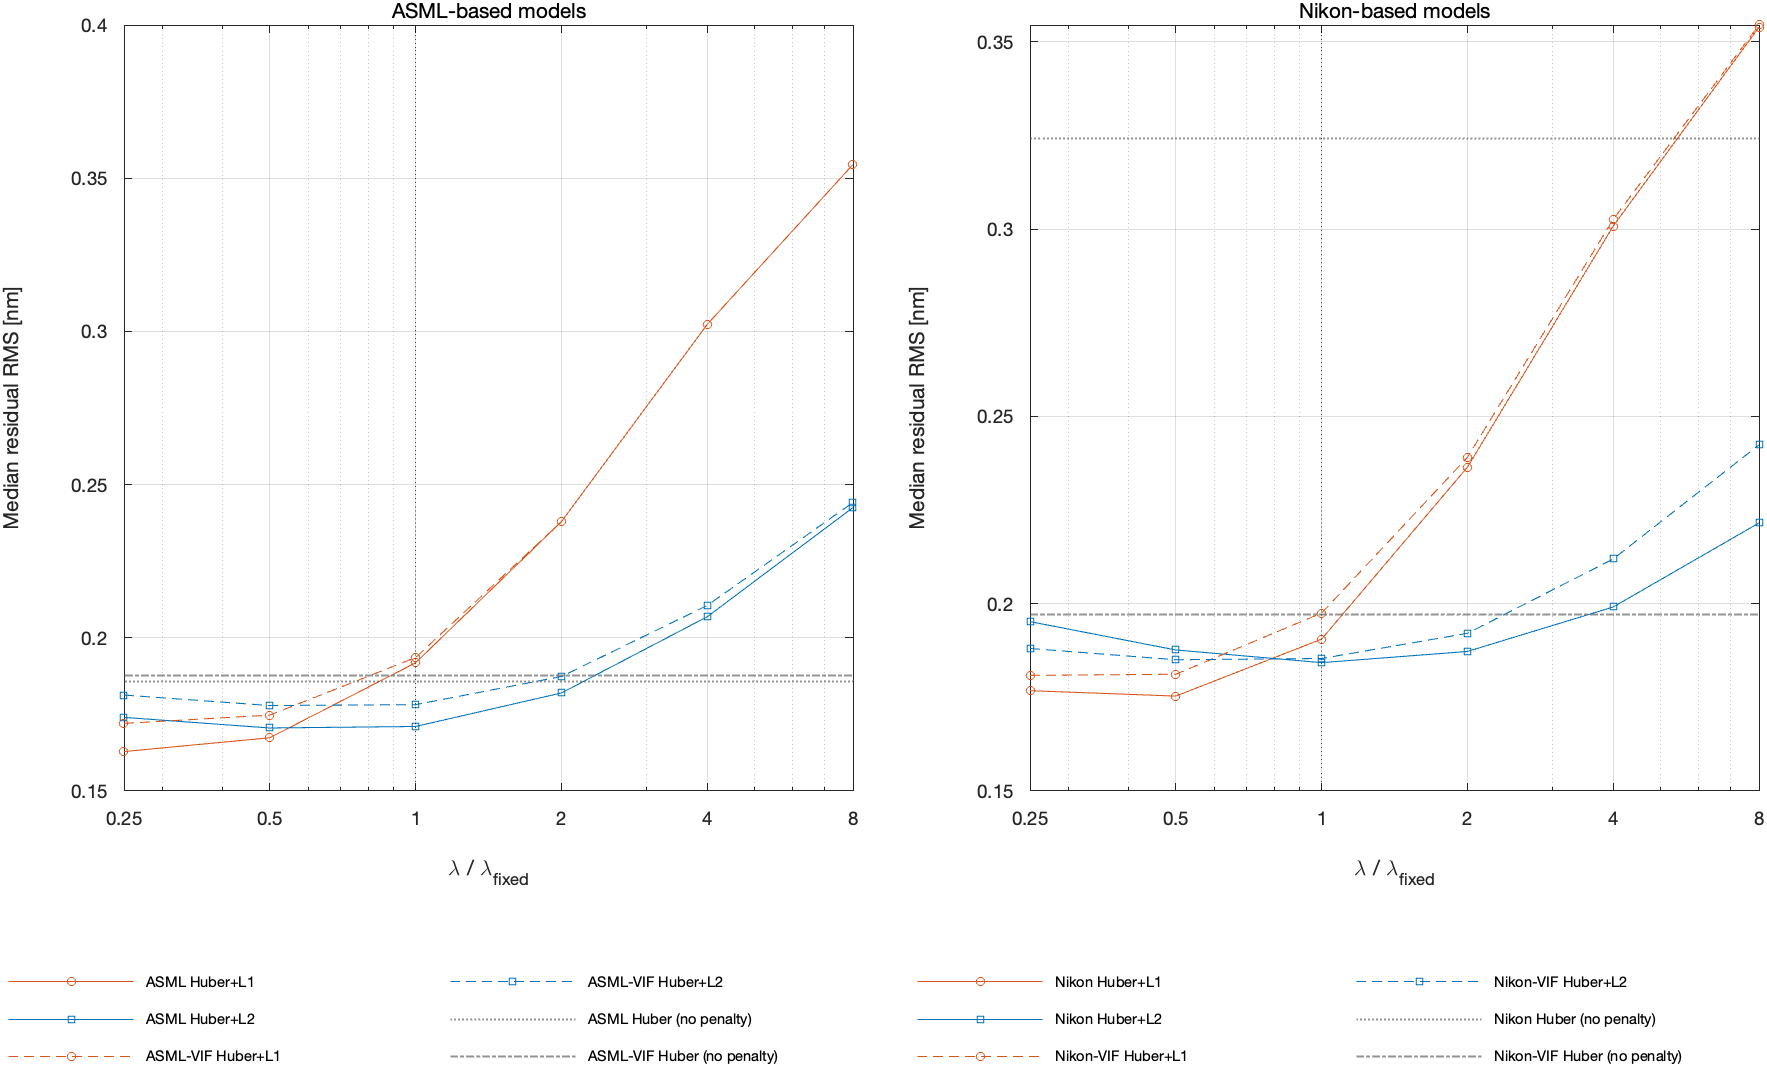
\includegraphics[width=\linewidth]{figures/fig_lambda_sweep}
  \caption{正則化の強さλを固定値の0.25〜8倍に変えたときの補正残差RMSの中央値（異常値あり，$d_x$と$d_y$の二乗平均）．左がASML系，右がニコン系の補正式．実線は削除前，破線はVIF削除後，灰色の点線と一点鎖線は罰則なしのHuber回帰を表す．}
  \label{fig:lambda}
\end{figure}

\subsection{測定点での残差によるモデル評価の危険性}

異常値なしの条件における補正残差と，測定点での見かけの残差（測定値と補正値の差のRMS）を表\ref{tab:clean}に示す．
ニコン式のOLSは，$d_y$の見かけの残差がASML式より小さい（0.231\,nmと0.256\,nm）にもかかわらず，Shot全面の残差は大きかった（0.253\,nmと0.157\,nm）．
項数を増やすと測定点での当てはまりは必ず良くなるため，測定点の残差だけで補正式を選ぶとオーバーフィッティングを見逃す．
測定していない位置での誤差を見積もる交差検証\cite{Ehrlich2025}や，本報告のようなシミュレーションによる評価が必要である．

また，異常値なしの条件では，すべての補正式でL2の残差が最も小さく，ニコン式（削除前）でもL2を用いれば0.152〜0.157\,nmと，ASML式のOLS（0.152〜0.157\,nm）と同等になった．
正則化によって，項数の多い補正式でも表現力を保ったまま分散を抑えられることを示している．

\begin{table}[tb]
  \centering
  \caption{異常値なしの条件における補正残差と，測定点での見かけの残差のRMSの中央値 [nm]．太字は各補正式の中でShot全面の残差が最小の手法を表す．}
  \label{tab:clean}
  \small
  \begin{tabular}{llcccc}
    \toprule
     & & \multicolumn{2}{c}{Shot全面の残差} & \multicolumn{2}{c}{測定点での見かけの残差} \\
    \cmidrule(lr){3-4}\cmidrule(lr){5-6}
    補正式 & 手法 & $d_x$ & $d_y$ & $d_x$ & $d_y$ \\
    \midrule
    ASML & OLS & 0.152 & 0.157 & 0.251 & 0.256 \\
    (10/10) & Huber & 0.157 & 0.162 & 0.253 & 0.259 \\
     & L2 & \textbf{0.143} & \textbf{0.147} & 0.262 & 0.267 \\
     & L1 & 0.157 & 0.166 & 0.295 & 0.302 \\
     & Huber+L2 & 0.147 & 0.152 & 0.268 & 0.274 \\
     & Huber+L1 & 0.171 & 0.180 & 0.308 & 0.315 \\
    \midrule
    ASML-VIF & OLS & 0.155 & 0.161 & 0.264 & 0.269 \\
    (9/9) & Huber & 0.158 & 0.166 & 0.267 & 0.271 \\
     & L2 & \textbf{0.150} & \textbf{0.156} & 0.271 & 0.276 \\
     & L1 & 0.160 & 0.168 & 0.296 & 0.302 \\
     & Huber+L2 & 0.153 & 0.162 & 0.277 & 0.281 \\
     & Huber+L1 & 0.172 & 0.181 & 0.309 & 0.315 \\
    \midrule
    Nikon & OLS & 0.230 & 0.253 & 0.247 & 0.231 \\
    (12/15) & Huber & 0.239 & 0.265 & 0.253 & 0.237 \\
     & L2 & \textbf{0.152} & \textbf{0.157} & 0.267 & 0.261 \\
     & L1 & 0.161 & 0.161 & 0.298 & 0.291 \\
     & Huber+L2 & 0.157 & 0.160 & 0.273 & 0.266 \\
     & Huber+L1 & 0.173 & 0.174 & 0.308 & 0.303 \\
    \midrule
    Nikon-VIF & OLS & 0.162 & 0.165 & 0.278 & 0.260 \\
    (8/10) & Huber & 0.166 & 0.170 & 0.280 & 0.262 \\
     & L2 & \textbf{0.160} & \textbf{0.154} & 0.284 & 0.270 \\
     & L1 & 0.167 & 0.165 & 0.304 & 0.299 \\
     & Huber+L2 & 0.164 & 0.160 & 0.288 & 0.275 \\
     & Huber+L1 & 0.178 & 0.178 & 0.315 & 0.312 \\
    \bottomrule
  \end{tabular}
\end{table}

\subsection{本検討の限界}

\begin{itemize}
  \item 真の歪みの係数分布（表\ref{tab:truth}）は仮定である．特に$y^4$〜$y^6$などの高次成分が実際にどの程度存在するかによって，事前削除の損得は変わるため，実データでの係数分布の把握が必要である．
  \item ニコン式の項構成は，係数名の添字を次数と解釈して作成したものであり，装置仕様との照合が必要である．
  \item マーク配置は$5\times7$点の1通りのみである．VIFはマーク配置で決まるため，マーク数や配置が変われば削除される項も変わる．
  \item Shotは互いに独立に生成しており，ウェハ内・ロット間の相関や，R2R制御での係数の平滑化は考慮していない．
  \item ハイパーパラメータは固定値であり，交差検証による調整や，L1で選択した後の再当てはめは評価していない．
\end{itemize}

% ============================================================
\section{結論}
% ============================================================

本報告では，Shot高次補正の回帰計算で生じる異常値，測定誤差，多重共線性，オーバーフィッティングの課題に対し，VIFによるkパラメータの事前選定，Huber回帰，正則化を組み合わせる手法を提案した．
ASML式とニコン式を題材に，乱数で生成した1000通りのShotで評価し，次の結論を得た．

\begin{enumerate}
  \item \textbf{kパラメータの事前削除は，L1正則化を用いる場合でも条件によって有効である．}
        ロバスト回帰を併用しないL1では，事前削除により残差の中央値が2.4〜4.5\,\%低減した．
        正則化を用いない場合の効果はさらに大きく，ニコン式で39〜44\,\%低減した．
        一方，Huber回帰とL1を併用した場合は残差の改善は見られなかった（$-0.9$〜$-3.7$\,\%）．
        この条件での事前削除の意義は，残差の低減よりも共線性による係数の不安定化を防ぐ点にあると考えられ，ロット間の係数変動を含めた検証が今後の課題である．
  \item \textbf{事前に削除した補正式では，L1正則化よりL2正則化が有効である．}
        Huber回帰と組み合わせた場合，L2はL1より残差の中央値が6.1〜7.9\,\%小さく（勝率68.8〜70.1\,\%），異常値なしの条件でも5.8〜11.3\,\%小さかった．
        L2はλの設定がずれても性能が崩れにくく，λを固定して運用する量産の補正に適する．
        ただし，λを小さく調整した場合にはL1がわずかに優れた．
  \item \textbf{ロバスト回帰の効果が最も大きい．}
        異常値を含む条件で，Huber回帰は最小二乗法に対して残差の中央値を66〜69\,\%低減し，約90\,\%のShotで改善した．
        異常値を含まない条件での損失は2.5〜4.2\,\%にとどまった．
\end{enumerate}

以上から，Shot高次補正の回帰では，まずロバスト回帰を導入し，そのうえでL2正則化によって係数の分散を抑える構成を推奨する．
VIF削除と組み合わせたこの構成により，現行の最小二乗法に比べて残差の中央値はASML式で70\,\%，ニコン式で82\,\%低減した．
正則化を用いない場合には，VIFによるkパラメータの事前削除が不可欠である．

% ============================================================
\section*{謝辞}
\addcontentsline{toc}{section}{謝辞}
% ============================================================
本報告の作成にあたり，有益な議論と助言をいただいた関係者の皆様に感謝いたします．  % ← 必要に応じて書き換える

% ============================================================
% 参考文献（本文で最初に引用した順）
% ============================================================
\clearpage
\phantomsection
\addcontentsline{toc}{section}{参考文献}
\begin{thebibliography}{99}

\bibitem{Adel2007}
M. Adel, P. Izikson, D. Tien, C. K. Huang, J. C. Robinson, and B. Eichelberger,
``The challenges of transitioning from linear to high-order overlay control in advanced lithography,''
Proc. SPIE \textbf{6827}, 682722 (2007). doi:10.1117/12.778457

\bibitem{Gabor2026}
A. Gabor, M. Burkhardt, D. Goldfarb, L. Meli, and J. Rankin,
``IBM lithography roadmap: shorter-wavelength lithography, resist and mask requirements to reduce stochastic defects,''
Proc. SPIE \textbf{13979}, 139790R (2026). doi:10.1117/12.3091000

\bibitem{Klein2026}
D. Klein and N. Gutman,
``Overlay metrology performance specification challenge entering the sub-nanometer overlay era,''
Proc. SPIE \textbf{13981}, 139813L (2026). doi:10.1117/12.3090660

\bibitem{Katz2026}
S. Katz, P. Leray, H. Yang, Y. Cho, V. Blanco, R. Gronheid, E. Megged, and Y. Grauer,
``Optical overlay metrology challenges in next-gen semiconductor nodes,''
Proc. SPIE \textbf{13981}, 139811A (2026). doi:10.1117/12.3090568

\bibitem{MacMillen1982}
D. MacMillen and W. D. Ryden,
``Analysis of image field placement deviations of a 5x microlithographic reduction lens,''
Proc. SPIE \textbf{334}, 78 (1982). doi:10.1117/12.933563

\bibitem{Duclaux2020}
B. Duclaux, M. Gatefait, O. Mermet, and J.-D. Chapon,
``Run to run and model variability of overlay high order process corrections for mean intrafield signatures,''
Proc. SPIE \textbf{11325}, 113251K (2020). doi:10.1117/12.2551062

\bibitem{Huang2012FxFc}
C.-Y. Huang, C.-F. Chiu, W.-B. Wu, C.-L. Shih, C.-C. K. Huang, H. Huang, D. Choi, B. Pierson, and J. C. Robinson,
``Overlay control methodology comparison: field-by-field and high-order methods,''
Proc. SPIE \textbf{8324}, 832427 (2012). doi:10.1117/12.916427

\bibitem{Lim2014}
M. Lim, G. Kim, S. Kim, B. Lee, S. Kim, C. Lim, M. Kim, and S. Park,
``Investigation on reticle heating effect induced overlay error,''
Proc. SPIE \textbf{9050}, 905014 (2014). doi:10.1117/12.2048281

\bibitem{Pike2015}
M. Pike, T. Brunner, B. Morgenfeld, N. Jing, and T. Wiltshire,
``Intra-field overlay correction for illumination based distortion,''
Proc. SPIE \textbf{9426}, 942613 (2015). doi:10.1117/12.2085887

\bibitem{Matsuyama2015}
T. Matsuyama,
``Exposure tool control for advanced semiconductor lithography,''
Adv. Opt. Technol. \textbf{4}(4), 285--296 (2015). doi:10.1515/aot-2015-0026

\bibitem{Ishiyama2016}
S. Ishiyama, Y. Ohmura, Y. Tsuge, T. Hirayama, H. Ikezawa, D. Inoue, Y. Kitamura, Y. Koizumi, K. Hasegawa, T. Nakashima, T. Kikuchi, M. Onda, Y. Takase, A. Nagahiro, S. Isago, and H. Kawahara,
``High-order aberration control during exposure for leading-edge lithography projection optics,''
Proc. SPIE \textbf{9780}, 97800Y (2016). doi:10.1117/12.2218840

\bibitem{Chen2018}
C. Chen, E. C. Lio, H. L. Hsu, J. H. Chang, S. S. Lee, P. Lomtscher, B. Habets, G. Erley, N. Birnstein, S. Tottewitz, and R. Liu,
``Higher order intra-field alignment for intra-wafer lens and reticle heating control,''
Proc. SPIE \textbf{10585}, 105851R (2018). doi:10.1117/12.2297358

\bibitem{Huang2009}
C. Y. Huang, C. F. Chue, A.-H. Liu, W. B. Wu, C. L. Shih, T.-B. Chiou, J. Lee, O. Chen, and A. Chen,
``Using intra-field high order correction to achieve overlay requirement beyond sub-40nm node,''
Proc. SPIE \textbf{7272}, 72720I (2009). doi:10.1117/12.813628

\bibitem{Chiu2012}
C.-F. Chiu, C.-Y. Huang, J. Shieh, T.-B. Chiou, A. Li, C.-L. Shih, and A. Chen,
``Impacts of overlay correction model and metrology sampling scheme on device yield,''
Proc. SPIE \textbf{8324}, 83241S (2012). doi:10.1117/12.916601

\bibitem{Rui2025}
D. Rui, L. Zhang, Y. Wei, and Y. Su,
``Method of high-order advanced lithography overlay correction to enhance the manufacturing performance of integrated circuits,''
Nanoscale Adv. \textbf{7}, 6563--6574 (2025). doi:10.1039/d5na00682a

\bibitem{Ullah2013}
M. Z. Ullah, M. F. M. Jazim, S. Tran, A. Qiu, D. Goh, J. Ang, D. Goh, D. Tien, K. Huang, and D. Choi,
``An investigation of high-order process correction models and techniques to improve overlay control by using multiple-pass cascading analysis at an advanced technology node,''
Proc. SPIE \textbf{8681}, 86813A (2013). doi:10.1117/12.2011448

\bibitem{Ju2016}
J. Ju, M. Kim, J. Lee, J. Nabeth, S. Jeon, H. Heo, J. C. Robinson, and B. Pierson,
``Application of overlay modeling and control with Zernike polynomials in an HVM environment,''
Proc. SPIE \textbf{9778}, 977825 (2016). doi:10.1117/12.2219739

\bibitem{Ehrlich2025}
C. Ehrlich, P. Groeger, U. Denker, S. Boese, and S. Jung,
``Cherry-picking: automated model term selection for precise overlay and CD process control,''
Proc. SPIE \textbf{13426}, 134260U (2025). doi:10.1117/12.3051064

\bibitem{Ehrlich2026}
C. Ehrlich, U. Denker, P. Gr\"{o}ger, G. de Liedekerke Beaufort, X. Thrun, T. Taylor, V. Temchenko, and R. Khurana,
``Smart Zernike: automated model term selection for enhanced track module matching and CDU control in photolithography,''
Proc. SPIE \textbf{13981}, 139812V (2026). doi:10.1117/12.3090707

\bibitem{Mohammad2026}
S. N. Mohammad, C. Utzny, A. Lopez-Gomez, S. Boese, and P. Groeger,
``Leveraging principal component analysis for overlay variation and root cause discovery in high-volume manufacturing,''
Proc. SPIE \textbf{13981}, 139813U (2026). doi:10.1117/12.3090685

\bibitem{Tibshirani1996}
R. Tibshirani,
``Regression shrinkage and selection via the lasso,''
J. R. Stat. Soc. B \textbf{58}(1), 267--288 (1996).

\bibitem{Lee2017}
H. Lee, S. Han, J. Woo, D. Lee, C. Song, H. Heo, I. Brinster, D. Choi, and J. C. Robinson,
``High-volume manufacturing device overlay process control,''
Proc. SPIE \textbf{10145}, 101450D (2017). doi:10.1117/12.2257836

\bibitem{Marquardt1970}
D. W. Marquardt,
``Generalized inverses, ridge regression, biased linear estimation, and nonlinear estimation,''
Technometrics \textbf{12}(3), 591--612 (1970).

\bibitem{Huber1964}
P. J. Huber,
``Robust estimation of a location parameter,''
Ann. Math. Statist. \textbf{35}(1), 73--101 (1964).

\bibitem{Holland1977}
P. W. Holland and R. E. Welsch,
``Robust regression using iteratively reweighted least-squares,''
Commun. Stat. Theory Methods \textbf{6}(9), 813--827 (1977).

\bibitem{Hoerl1970}
A. E. Hoerl and R. W. Kennard,
``Ridge regression: biased estimation for nonorthogonal problems,''
Technometrics \textbf{12}(1), 55--67 (1970).

\bibitem{Friedman2010}
J. Friedman, T. Hastie, and R. Tibshirani,
``Regularization paths for generalized linear models via coordinate descent,''
J. Stat. Softw. \textbf{33}(1), 1--22 (2010).

\bibitem{Zou2005}
H. Zou and T. Hastie,
``Regularization and variable selection via the elastic net,''
J. R. Stat. Soc. B \textbf{67}(2), 301--320 (2005).

\end{thebibliography}

\end{document}
